\section{Evaluation and Discussion}
\label{sec:discussion}

\begin{figure}[t]
\centering
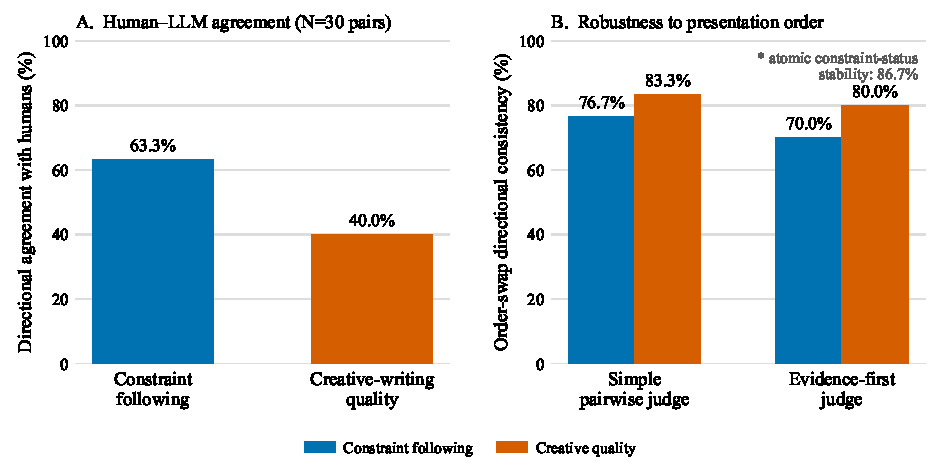
\includegraphics[width=\linewidth]{figures/figure_evaluator_validity.pdf}
\caption{Evaluator validity, over the fixed N=30 blind human-annotated sample (\cref{sec:human_eval}). \textbf{(A)} Directional agreement between the simple pairwise LLM evaluator and human judgments, separately for constraint following and creative-writing quality. \textbf{(B)} Order-swap directional consistency (primary vs.\ orientation-restored reversed judgment) for the simple pairwise evaluator and the evidence-first evaluator, separately for constraint following and creative quality; the starred annotation is the evidence-first evaluator's atomic constraint-status stability (430/496 individual satisfied/partial/violated decisions stable under reversal, 86.7\%) --- a different, more granular quantity than the adjacent bars, not a fifth bar on the same scale. Quadratic-weighted Cohen's kappa is not shown on these axes because it is not commensurable with a percentage; see \cref{tab:human_alignment}.}
\label{fig:evaluator_validity}
\end{figure}

\begin{table}[t]
\centering
\small
\begin{tabular}{lrr}
\toprule
\textbf{Dimension} & \textbf{Directional agreement} & \textbf{Quadratic-weighted $\kappa$} \\
\midrule
Constraint following     & 63.3\% & 0.544 \\
Creative-writing quality & 40.0\% & 0.078 \\
\bottomrule
\end{tabular}
\caption{Human--model agreement for the simple pairwise LLM evaluator, N=30 blind pairs (\cref{sec:human_eval}). Quadratic-weighted Cohen's $\kappa$ measures chance-corrected agreement on the ordinal five-level preference scale.}
\label{tab:human_alignment}
\end{table}

\subsection{Human Alignment}
\label{sec:disc_human}

We compare human judgments against the simple pairwise LLM evaluator on the fixed, stratified sample of 30 FULL/Sharded pairs described in \cref{sec:human_eval}: each of the six models and each of the six genres appears in five cases, with coverage of a range of automated-score relationships hidden from annotators. Three human annotators each rated 10 non-overlapping pairs, so every case received exactly one human judgment and no case was double-rated. Annotators saw the same blinded, order-randomized Response A/Response B presentation given to both pairwise LLM evaluators, and rendered the same five-level categorical preference the simple pairwise evaluator uses, separately for constraint following and for creative-writing quality.

The simple pairwise evaluator's judgments align with this independent human preference far more strongly on constraint following than on holistic creative-writing quality. Directional agreement is 63.3\% for constraint following versus only 40.0\% for creative-writing quality (\cref{fig:evaluator_validity}A). On the full five-level ordinal scale, quadratic-weighted Cohen's $\kappa$ is $\kappa = 0.544$ for constraint following and $\kappa = 0.078$ for creative-writing quality (\cref{tab:human_alignment}) --- moderate agreement on the former and close to chance-level agreement on the latter. Severe disagreement (a human--model gap of at least three ordinal levels on the five-level scale) is rare for constraint following (3 of 30 cases) but affects nearly a third of cases for creative-writing quality (8 of 30 cases, 26.7\%). This comparison does not directly validate the pointwise judge used for the large-scale analysis. Instead, it provides evidence that, in our evaluation setting, holistic LLM judgments of literary quality are substantially less aligned with human preference than judgments of explicit constraint following.

\subsection{Judge Robustness}
\label{sec:disc_robustness}

Both pairwise LLM evaluators are reasonably self-consistent under order-swapping at the level of their final, aggregated preference. Under the simple pairwise protocol, primary and orientation-restored reversed judgments agree in direction 76.7\% of the time for constraint following and 83.3\% for creative quality; under the evidence-first protocol the corresponding figures are 70.0\% and 80.0\% (\cref{fig:evaluator_validity}B). At that aggregated level, creative-quality judgments are, if anything, slightly more order-stable than constraint judgments for both evaluators. The comparison inverts once each judgment is decomposed into its individual, item-level decisions. The evidence-first evaluator's atomic constraint-status audits (satisfied/partial/violated, one decision per response per constraint) are stable under order-swapping in 430 of 496 decisions, 86.7\% (\cref{fig:evaluator_validity}B, starred). Its eight per-dimension creative-quality winner judgments (prose and craft, coherence and progression, originality of execution, natural constraint integration, characterization, atmosphere and effect, narrative payoff, genre effectiveness) are individually far less stable, ranging from 60.0\% to 83.3\% winner-consistency across dimensions and averaging well below the atomic constraint figure. At matched granularity, then, fine-grained literary judgment is less stable under reversal than fine-grained constraint judgment. The higher stability of the final holistic preference should therefore not be interpreted as evidence that its underlying literary assessments are equally stable; several component judgments change substantially under response-order reversal. It is this granular gap, together with the human-alignment gap in \cref{sec:disc_human}, that makes constraint scoring the more defensible of the two: it is corroborated by both fine-grained self-consistency and independent human agreement, while holistic creative-quality scoring is comparatively unstable at the level its judgments are actually formed and only weakly corroborated by human agreement.

These results support using the automated evaluator as a scalable measure of explicit constraint satisfaction, while requiring greater caution when interpreting automated creative-quality scores as proxies for human literary preference.

\subsection{Interpretation}
\label{sec:disc_interpretation}

\paragraph{Multi-turn specification hurts global narrative organization beyond simple constraint loss.} RQ1 (\cref{sec:rq1}) shows a large adherence drop under Sharded, consistent with the broader ``getting lost in conversation'' literature: models are worse at satisfying explicit requirements when those requirements arrive one shard at a time. If observed constraint loss accounted for the entire structure/coherence difference, we would expect that gap to attenuate substantially among equal-adherence pairs. It does not. RQ3 (\cref{sec:rq3}) shows structure/coherence remains substantially worse for Sharded even among pairs where FULL and Sharded satisfied the same fraction of constraints. Forgetting or failing to satisfy individual requirements is therefore not sufficient to explain the full degradation. This persistence suggests that observed constraint loss alone is insufficient to account for the structure/coherence gap; progressive specification is associated with an additional loss in global narrative organization even among pairs with equal observed adherence. We take this to be the paper's main interpretive result: constraint adherence and narrative coherence emerge as distinct dimensions of multi-turn degradation rather than the same failure measured twice.

\paragraph{The effect is multidimensional rather than a uniform collapse in ``creativity.''} RQ2 (\cref{sec:rq2}) does not show Sharded losing across the board. FULL improves structure/coherence, craft, and genre effectiveness overall, but Sharded scores slightly higher on automated originality, and at equal adherence (RQ3) craft's advantage disappears entirely while originality, genre effectiveness, and characterization all shift toward Sharded. Originality is the dimension that stands out most: it is the only quality dimension where Sharded outscores FULL even in the full, non-equal-adherence comparison, so the larger SHARDED advantage at equal adherence sharpens an effect that was already present. Characterization, by contrast, warrants the opposite caution: its overall FULL advantage was small to begin with (\cref{sec:rq2}) and did not hold up when the analysis was restricted to same-judge-backend pairs (\cref{sec:limitations}), so we do not treat it as a reliably established effect in either direction. A single ``multi-turn makes writing worse'' story does not fit this pattern; a more cautious reading is that progressive interaction may preserve or increase rubric-scored originality even as global narrative organization degrades. We say \emph{may} deliberately: the originality result rests entirely on the automated judge, and \cref{sec:disc_human} shows that judge's agreement with human holistic-quality preference is weak, so a small LLM-judged originality edge for Sharded is not yet evidence of a real creative advantage.

\paragraph{Evaluating creative writing is itself part of the problem.} The judge-validation results in \cref{sec:disc_human,sec:disc_robustness} are not a side note to the RQ1--RQ3 findings; they qualify how much weight those findings can bear. Explicit constraints are comparatively concrete, and the simple pairwise evaluator's constraint-following judgments agree reasonably well with human preference. Qualities such as atmosphere, emotional gravity, and literary depth appear less stable in the LLM order-swap audits and show substantially weaker human--LLM agreement than explicit constraint satisfaction. One disagreement in the human-validation sample illustrates the gap concretely: for a pair of stories about a field-hospital nurse, the human reviewer strongly preferred the longer response, citing how it ``masterfully conveys the raw emotions'' and the ``cruel and constricting conditions,'' and judged the shorter alternative to lack ``the gravity'' and ``punches'' of the first, despite the shorter response satisfying the stated constraints more precisely. The simple pairwise evaluator preferred the shorter response for creative quality, with the stated justification that it was ``more economical and focused.'' One case does not establish a general rule, but it makes the weak human--LLM creative-quality agreement in \cref{sec:disc_human} concrete rather than abstract: the judge and the human reviewer were not making the same kind of comparison at all.

\subsection{Comparison with Prior Work}
\label{sec:disc_prior_work}

Earlier multi-turn degradation studies largely evaluate objectively checkable requirements: word counts, exact phrases, code that passes or fails a test, dialogue turns that either recall or forget an established fact \citep{laban2025llmslostmultiturnconversation,he2024multiifbenchmarkingllmsmultiturn,jia2026battleanotherprobingllms,li2025structflowbenchstructuredflowbenchmark}. Even SEQUOR, the benchmark closest to ours, explicitly filters out constraints judged subjective before measuring how accuracy drops as constraints accumulate across turns \citep{canaverde2026sequormultiturnbenchmarkrealistic}. Our results suggest that extending this setting to open-ended creative writing reveals two problems at once, not one: models must maintain evolving narrative state across turns, the same difficulty verifiable-task benchmarks already document, and evaluators must judge qualities for which no single objective target exists, a difficulty those benchmarks avoid by design. A benchmark that only measured the first problem, as ours would if it stopped at RQ1's adherence numbers, would understate how unsettled the creative-writing case still is.
